\section{Project Description}
\label{sec:project-description}

This section is written for product managers, designers, developers, marketing teams and AI-assisted landing-page generators. Every product claim is grounded in the repository; anything inferred is labelled as such.

\subsection{Product identity}
\status{IMPLEMENTED}

\begin{table}[H]
\centering
\caption{Product identity attributes extracted from the repository}
\label{tab:product-identity}
\begin{tabular}{@{}L{4.2cm}L{10.0cm}@{}}
\toprule
\textbf{Attribute} & \textbf{Value (evidence)} \\
\midrule
Working title & Learning Management System (\pathref{README.md}, \pathref{CONTRACT.md}) \\
UI brand name & Edvanta (\pathref{frontend/index.html} title, \pathref{frontend/src/components/Footer.jsx}) \\
Tagline (literal) & ``Learn Your Way'' (\pathref{frontend/index.html} \code{<title>}) \\
Hero headline & ``Empower your future with structured learning and verified credentials.'' (\pathref{frontend/src/pages/HomePage.jsx}) \\
Meta description & ``LMS Portal -- structured courses, rigorous assessments and verified certificates.'' (\pathref{frontend/index.html}) \\
Product category & B2C/B2B Education Technology -- Learning Management System \\
Delivery model & Single-page web application (responsive, browser-based) \\
Licence claim & ``MIT License'' stated in \pathref{README.md}; \textbf{no LICENSE file exists} \\
\bottomrule
\end{tabular}
\end{table}

\subsection{Problem statement}
\status{INFERRED}

Derived from the solution implemented in code: online learning content, assessments, progress records and credentials are typically scattered across tools, making it difficult to run a complete learn$\rightarrow$assess$\rightarrow$certify cycle in one place. The repository exists to provide one platform where that full lifecycle is executed end-to-end (the lifecycle diagram is part of \pathref{README.md} and \pathref{CONTRACT.md}).

\subsection{Solution}
\status{IMPLEMENTED}

A role-based web platform where:

\begin{itemize}
    \item \textbf{Learners} discover courses, enrol, watch/read lessons, track progress, take quizzes, discuss, review, and earn printable certificates.
    \item \textbf{Instructors} author courses, order lessons, create quizzes with questions and answer keys, publish content, and review learner submissions.
    \item \textbf{Administrators} manage users, course categories and the course catalogue, and monitor platform data.
\end{itemize}

\noindent All authority (scoring, eligibility, ownership) is enforced server-side in the Spring Boot backend -- see Section~\ref{sec:authorization}.

\subsection{Target audience and personas}
\status{IMPLEMENTED (roles) / INFERRED (personas)}

The three user roles are implemented in code (\code{User.Role} enum in \pathref{backend/src/main/java/com/example/lms/entity/User.java}: \code{LEARNER}, \code{INSTRUCTOR}, \code{ADMIN}). Persona narratives below are \emph{inferred} from the seeded demo accounts in \pathref{backend/src/main/java/com/example/lms/config/DataInitializer.java} and \pathref{database/seed.sql}; no real customer research exists in the repository.

\begin{table}[H]
\centering
\caption{Personas inferred from seeded accounts and role capabilities}
\label{tab:personas}
\begin{tabular}{@{}L{2.6cm}L{3.6cm}L{8.0cm}@{}}
\toprule
\textbf{Persona} & \textbf{Seeded account} & \textbf{Goals supported by implemented features} \\
\midrule
Learner (Alex Learner) & \code{learner@example.com}, role LEARNER & Browse/enrol, complete lessons, pass quizzes, track progress, hold certificates, join discussions, review courses \\
Instructor (Sarah Instructor) & \code{instructor@example.com}, role INSTRUCT\-OR & Create and publish courses, manage lessons, author quizzes/questions, view learner submissions and scores \\
Administrator (Admin User) & \code{admin@example.com}, role ADMIN & Manage users and categories, delete any course, view all quiz attempts, administer the platform \\
\bottomrule
\end{tabular}
\end{table}

\subsection{Value proposition}
\status{IMPLEMENTED}

\begin{enumerate}
    \item \textbf{Complete lifecycle in one system} -- from registration to a downloadable certificate, verified by the end-to-end integration test.
    \item \textbf{Authoritative assessment} -- quiz scores are computed by the backend against stored answer keys; the client never determines pass/fail (\pathref{backend/src/main/java/com/example/lms/service/QuizService.java}).
    \item \textbf{Verifiable credentials} -- each certificate carries a unique code (\code{LMS-XXXXXXXX-NNNN}) and is only issued when 100\% of lessons are complete and every quiz is passed (\pathref{backend/src/main/java/com/example/lms/service/CertificateService.java}).
    \item \textbf{Instructor self-service authoring} -- courses, ordered lessons, quizzes and question banks are managed through the Instructor Studio UI without developer involvement.
    \item \textbf{Built-in coding practice} -- course-attached coding problems with an embedded OneCompiler editor (Section~\ref{sec:integrations}).
\end{enumerate}

\subsection{Core feature inventory}
\status{IMPLEMENTED}

\begin{table}[H]
\centering
\caption{Feature inventory with primary implementation evidence}
\label{tab:feature-inventory}
\begin{tabular}{@{}L{4.4cm}L{7.4cm}L{2.4cm}@{}}
\toprule
\textbf{Feature} & \textbf{Primary evidence} & \textbf{Status} \\
\midrule
Registration / login / logout (JWT) & \pathref{backend/src/main/java/com/example/lms/controller/AuthController.java}, \pathref{frontend/src/context/AuthContext.jsx} & IMPLEMENTED \\
Role-based dashboards & \pathref{frontend/src/components/} Learner, Instructor and Admin dashboards & IMPLEMENTED \\
Course catalogue, search, category filter & \pathref{backend/src/main/java/com/example/lms/controller/CourseController.java}, \pathref{frontend/src/pages/CourseCatalogPage.jsx} & IMPLEMENTED \\
Course CRUD + publish states & \pathref{backend/src/main/java/com/example/lms/service/CourseService.java}, InstructorDashboard & IMPLEMENTED \\
Lesson management + player & \pathref{backend/src/main/java/com/example/lms/controller/LessonController.java}, \pathref{frontend/src/components/LessonPlayer.jsx} & IMPLEMENTED \\
Enrollment / unenrolment (soft drop) & \pathref{backend/src/main/java/com/example/lms/service/EnrollmentService.java} & IMPLEMENTED \\
Progress tracking per lesson and course & \pathref{backend/src/main/java/com/example/lms/service/ProgressService.java} & IMPLEMENTED \\
Quizzes, question banks, timed attempts & \pathref{backend/src/main/java/com/example/lms/service/QuizService.java}, \pathref{frontend/src/components/QuizPage.jsx} & IMPLEMENTED \\
Discussions with threaded replies & \pathref{backend/src/main/java/com/example/lms/service/DiscussionService.java}, DiscussionList/DiscussionItem & IMPLEMENTED \\
Course feedback (1--5 rating, one per user) & \pathref{backend/src/main/java/com/example/lms/service/FeedbackService.java}, FeedbackForm & IMPLEMENTED \\
Certificates with eligibility rules & \pathref{backend/src/main/java/com/example/lms/service/CertificateService.java}, CertificateCard & IMPLEMENTED \\
Coding practice workspace (OneCompiler) & \pathref{frontend/src/components/practice/} & IMPLEMENTED (local dataset) \\
Category administration & \pathref{backend/src/main/java/com/example/lms/controller/CategoryController.java}, AdminDashboard & IMPLEMENTED \\
OpenAPI/Swagger documentation & \pathref{backend/src/main/java/com/example/lms/config/OpenApiConfig.java} & IMPLEMENTED \\
\bottomrule
\end{tabular}
\end{table}

\subsection{Product workflow}
\status{IMPLEMENTED}

\begin{figure}[H]
    \centering
    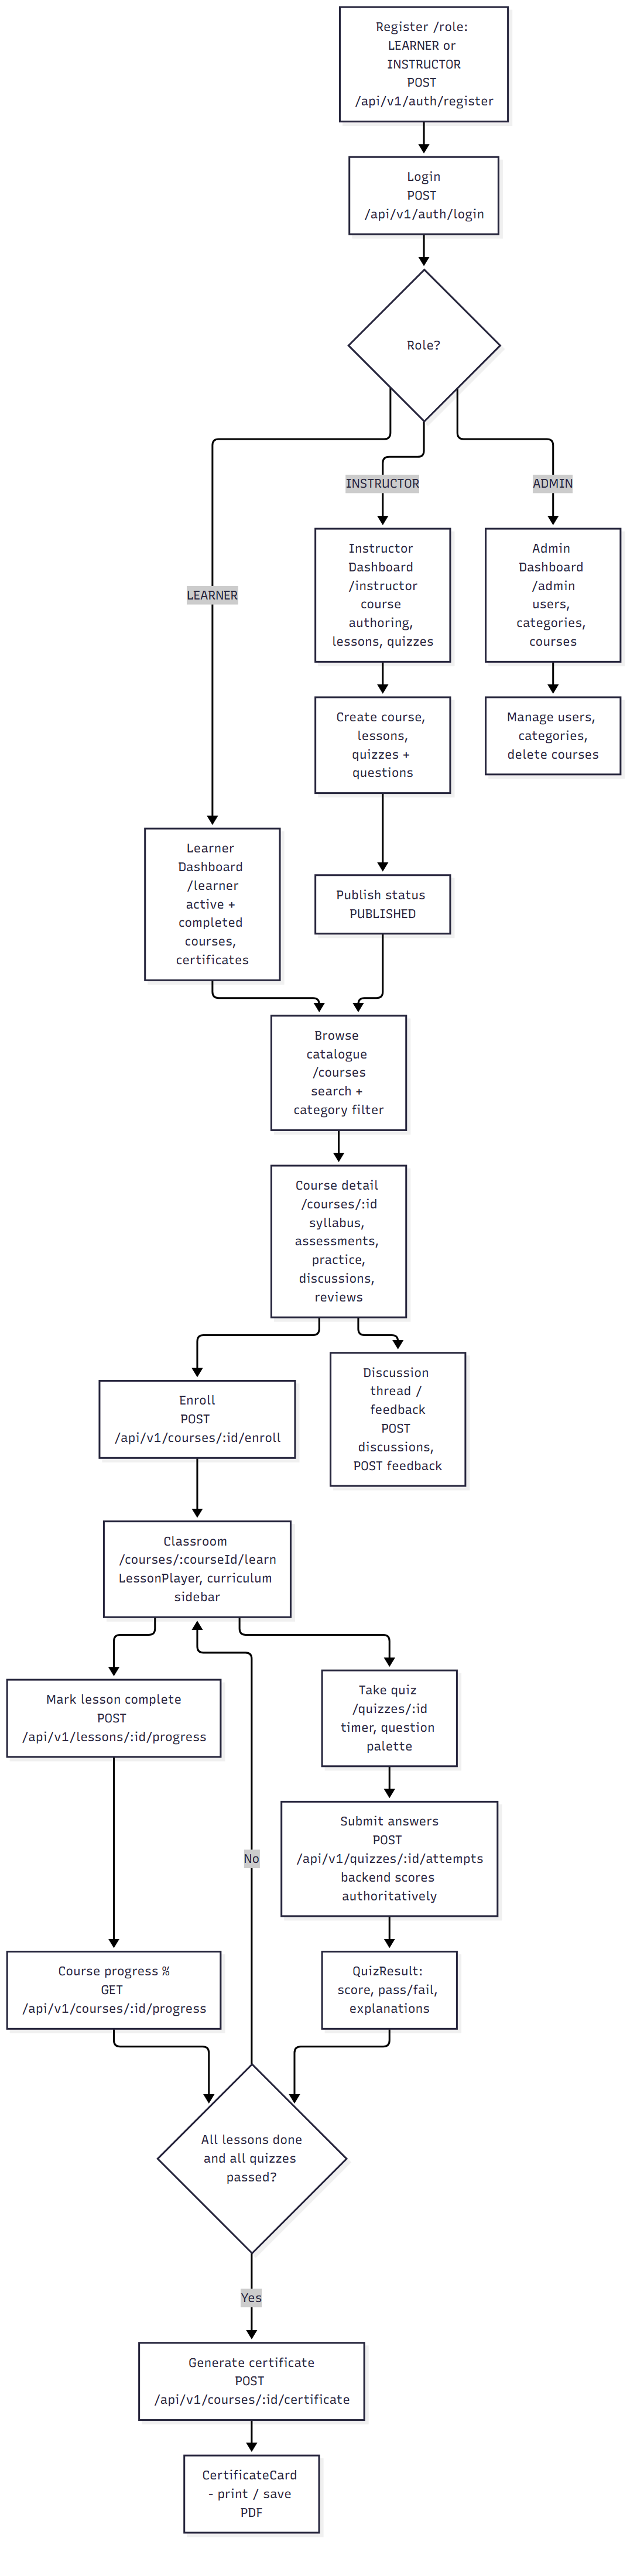
\includegraphics[width=0.86\textwidth]{diagrams/learning-lifecycle.png}
    \caption{Implemented product workflow -- learning lifecycle across the three roles}
    \label{fig:learning-lifecycle}
\end{figure}

\subsection{Use cases}
\status{IMPLEMENTED}

\begin{enumerate}
    \item \textbf{Self-paced learner}: registers, browses the catalogue, enrols, completes lessons in order, passes a timed quiz, and prints a certificate from the dashboard.
    \item \textbf{Instructor content author}: creates a course in draft, adds ordered lessons with video links or reading text, authors a quiz with answer keys, publishes, then reviews learner submissions and scores.
    \item \textbf{Platform administrator}: seeds and curates categories, reviews the user directory, removes courses, and audits all quiz attempts.
    \item \textbf{Practice learner}: opens \code{/practice} or a course's practice tab and solves coding problems inside the embedded OneCompiler editor against a static problem set.
\end{enumerate}

\subsection{Differentiators (repository evidence only)}
\status{IMPLEMENTED}

\begin{itemize}
    \item \textbf{Enforced certificate eligibility}: all lessons completed \emph{and} every quiz passed -- implemented server-side, tested in \pathref{CertificateServiceTest.java}.
    \item \textbf{Course-scoped coding practice}: static, versioned practice problems attached to real course IDs, with starter-code injection via \code{postMessage} into the OneCompiler iframe.
    \item \textbf{Engineering contract as product governance}: \pathref{CONTRACT.md} fixes ownership, API change control, and a Definition of Done -- unusual discipline for a project of this size.
\end{itemize}

\noindent \textbf{Not differentiators, honestly stated:} there is no recommendation engine, no payments, no mobile app, no video hosting, and no analytics -- all explicitly excluded in \pathref{CONTRACT.md} section 5.2.

\subsection{Calls to action present in the UI}
\status{IMPLEMENTED}

Home page (\pathref{frontend/src/pages/HomePage.jsx}): ``Browse all courses'' (primary), ``Join for free'' (logged-out) or ``Go to dashboard'' (logged-in), closing dark CTA band. Auth pages: ``Log in to Edvanta'', ``Create Your Account''. Course pages: ``Enroll Now'' / ``Continue Learning'' (\pathref{frontend/src/components/EnrollmentButton.jsx}). Additional CTA ideas are \status{RECOMMENDED} and intentionally not listed as product copy.

\subsection{Visual identity}
\status{IMPLEMENTED}

Brand gradient \texttt{linear-gradient(90deg, \#fc4c02 0\%, \#ef2cc1 52\%, \#bdbbff 100\%)} rendered by \pathref{frontend/src/components/ui/GradientRibbon.jsx}; black-first UI (\texttt{colorPrimary: \#000000}), mint accent \texttt{\#c8f6f9}, dark canvas \texttt{\#010120}. Full token tables are in Section~\ref{sec:design-system}.

\subsection{SEO keywords and AEO/GEO pointers}
\status{INFERRED (keywords) / IMPLEMENTED (metadata)}

Literal metadata supports the keywords ``LMS'', ``structured courses'', ``assessments'', ``certificates'', ``learn''. \status{RECOMMENDED} additional keyword families (``online learning platform'', ``course management system'') are \emph{not} present in the repository and must be added deliberately -- see Sections~\ref{sec:seo}, \ref{sec:aeo} and \ref{sec:geo} for the gap analysis.
